% !TEX root = ./main.tex
\chapter{Impacts of emissions spatial heterogeneity on aerosol properties and CCN activity}
%\chapter{Impacts of emissions spatial heterogeneity on aerosol properties in a particle resolved framework}

This chapter presents results for the impacts of emissions spatial heterogeneity on aerosol properties, including changes to the aerosol size distribution, composition, mixing state, and CCN activity. We begin with a set of simplified simulations to isolate the effect of spatial heterogeneity on an important aerosol process, coagulation. Subsequently, we present simulation results for full multiphase chemistry runs and discuss changes to aerosol properties and CCN activity. We find that under high emissions spatial heterogeneity, up to 25\% more CCN activate in the upper boundary layer for supersaturations in the range $S=0.3\%$ to $S=0.6\%$. 
\section{Idealized coagulation simulations}

Prior to discussing simulations utilizing the full multiphase chemical mechanism for aerosols and chemistry, we first focus our discussion on the impact of spatial heterogeneity on aerosol number concentration due to coagulation. Coagulation is a primary mechanism for aerosol aging and its rate scales with the square of the number concentration of particles, thus making it an important aerosol processes for which to evaluate the impacts of spatial heterogeneity. 

\subsection{Simulation scenarios}

\begin{figure}[h]
  \centering
    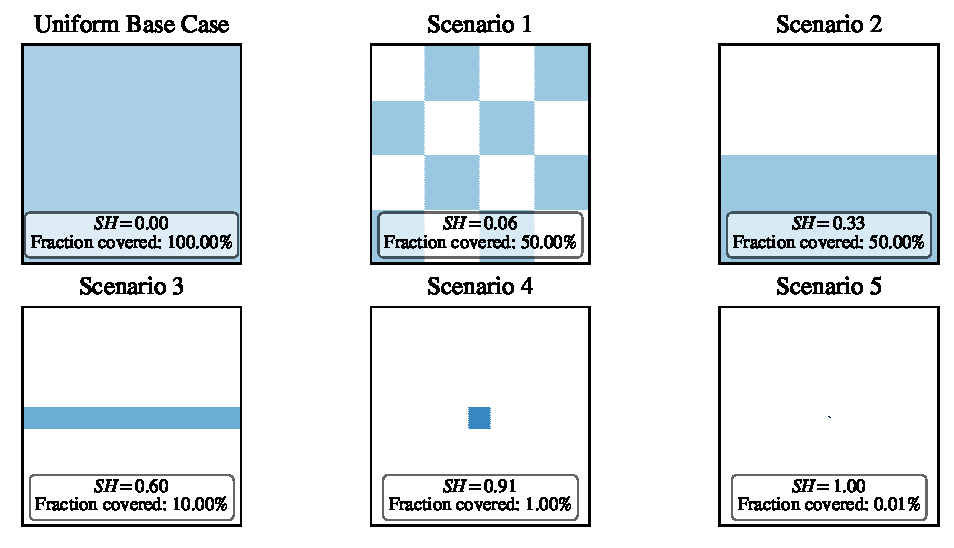
\includegraphics[width=\textwidth]{figures/chapter5/ideal-coag/ideal-coag-SH-scenarios.pdf}
    \caption{$SH$ scenarios for ideal coagulation simulations.}
    \label{fig:sh-scenarios-ideal-coag}
\end{figure}

Here we investigate the modification to the rate of coagulation under numerous spatial heterogeneity scenarios. We run a total of 6 simulations for a range of $SH$ scenarios shown in Figure \ref{fig:sh-scenarios-ideal-coag}. As with gas phase simulations in chapter 4, the concentration of atmospheric constituents (here aerosol particle number concentration) must be scaled within the $SH$ scenario region by the ratio of the area of the uniform base case and the area occupied by the $SH$ pattern. For example, the number concentrations in the central region of scenario 5 are a factor of 10,000 higher than in the uniform base case. 

Note that the setup of these simulations differs from all other simulations discussed in this thesis. Chemistry is turned off primarily for computational efficiency as, here, we are simply interested in changes to the number concentration rather than changes to aerosol composition. Rather than using initial conditions that are uniform throughout the domain, here the aerosol initial condition is set by the chosen $SH$ scenario for each vertical level in the domain (i.e., the pattern extends vertically throughout the domain). Additionally, emissions are turned off such that only coagulation is responsible for changes to aerosol number concentration.

\subsection{Results}

\begin{figure}[!h]
  \centering
    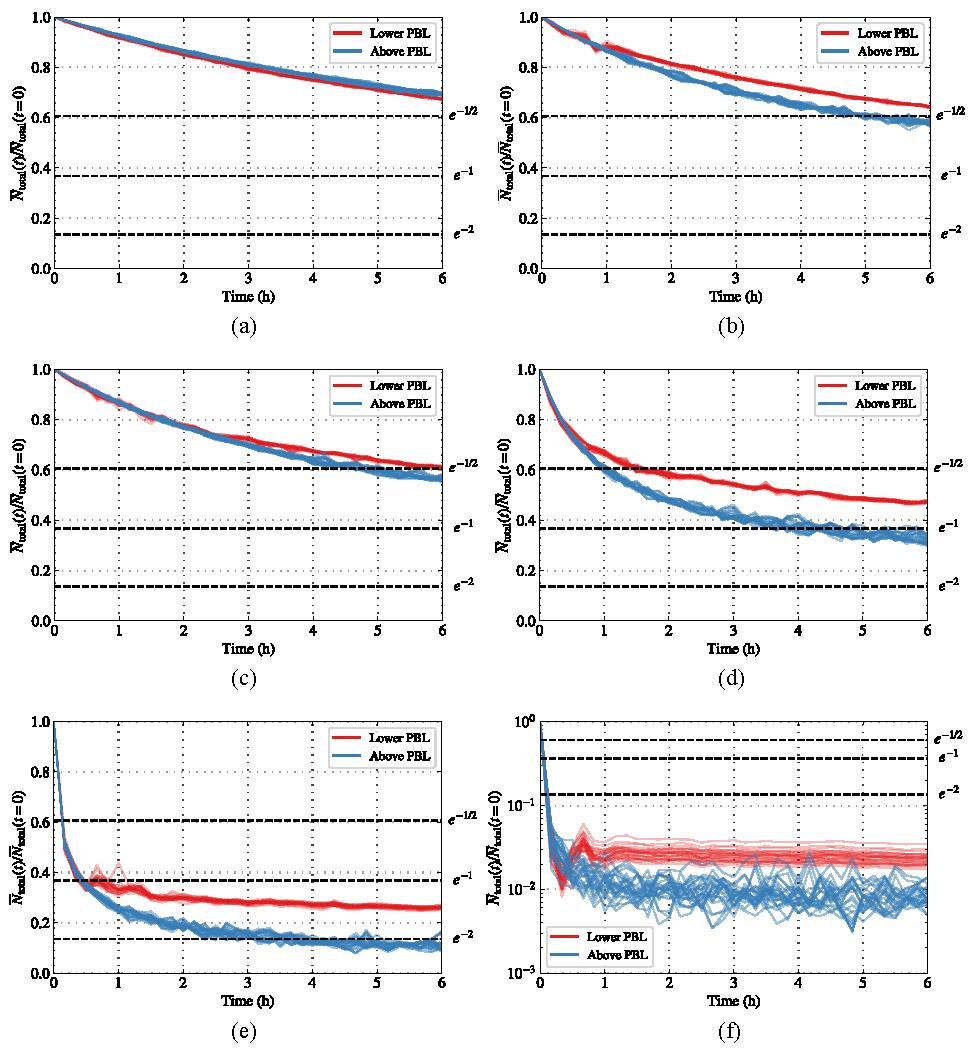
\includegraphics[width=\textwidth]{figures/chapter5/ideal-coag/NumConcTimescale_composite.pdf}
    \caption{Total number concentration for each $SH$ scenario normalized by the initial condition total number concentration. Lines indicate normalized number concentration averaged over each vertical level in the domain. (a) Uniform base case. (b--f) Scenarios 1--5}
    \label{fig:numconc-timescales}
\end{figure}

Figure \ref{fig:numconc-timescales} show how the total number concentration of aerosol particles decreases due to coagulation under each $SH$ scenario. For each scenario, we compute the average number concentration at each vertical level and time $t$, $\overline{N}_{\text{total}}(t)$. This number concentration is then normalized by the number concentration at time $t=0$, $\overline{N}_{\text{total}}(t=0)$. A subset of number concentration timeseries are shown in Figure \ref{fig:numconc-timescales} for the lowest 20 vertical levels of the PBL ($z=0$ m to $z\sim200$ m) and highest 20 vertical levels in the domain above the PBL ($z\sim1.8$ km to $z=2$ km). The reason for this grouping is that these two regions are notably different in terms of the rate at which the total number concentration decreases. For scenarios 1--5 (Figure \ref{fig:numconc-timescales} subfigures b--f), we find that the total number concentration decreases slower in the lower PBL than above the PBL. A notable exception to this trend is the uniform base case (Figure \ref{fig:numconc-timescales} subfigure a). Recall that the rate of coagulation scales as the square of the number of particles. As a result, highly heterogeneous patterns that require significant scaling up of the number concentration will have greater rates of coagulation within the high-concentration region associated with the $SH$ pattern. As the PBL develops and turbulent motion begins to diffuse the initial structure of the $SH$ pattern, concentration gradients are reduced, resulting in a reduction of the rate of coagulation. This turbulent motion does not disturb the structure of the $SH$ pattern above the PBL, and thus coagulation will proceed at a faster rate within the high concentration region of the $SH$ pattern.

We find that as the $SH$ increases across scenarios, the total number concentration is reduced more rapidly. For each plot in Figure \ref{fig:numconc-timescales}, we include horizontal dashed lines indicating the e-folding time alongside a half e-folding time ($e^{-1/2}$) and double e-folding time as the rate at which the total number concentration is reduced under $SH$ scenarios varies widely.  

\begin{figure}[t]
  \centering
    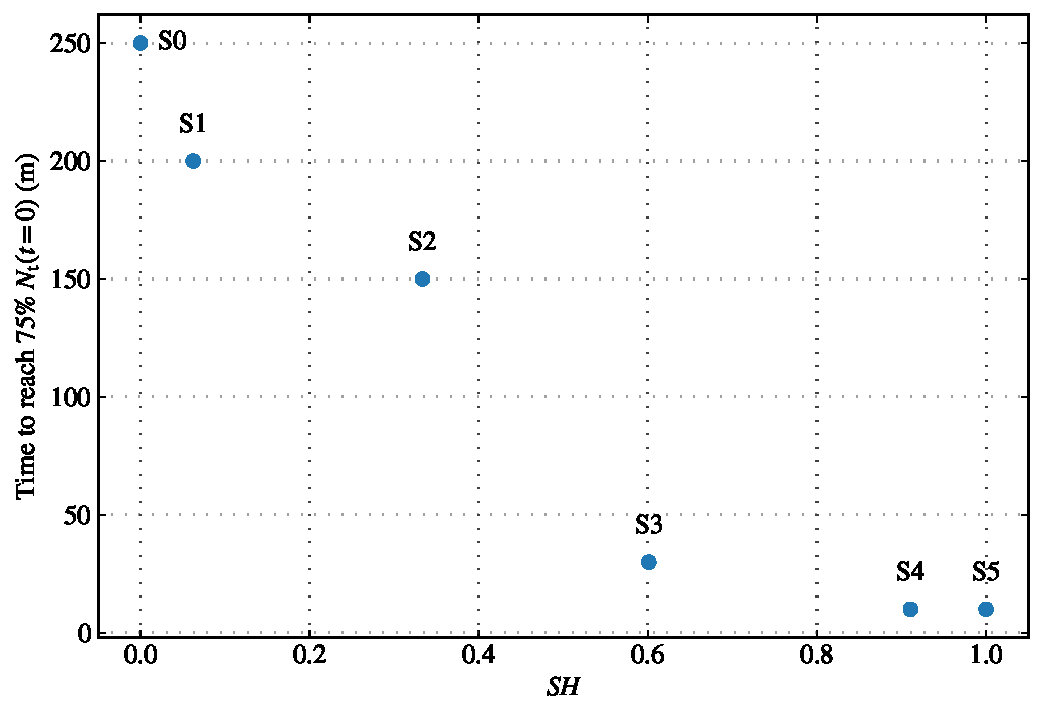
\includegraphics[width=\textwidth]{figures/chapter5/ideal-coag/TimeTo75pcnt_vs_SH.pdf}
    \caption{Time required in minutes for the total number concentration in the lowest 200 m of the PBL to be reduced to 75\% of the initial value vs. scenario $SH$. ``S0" is the uniform base case, with all other scenarios labeled S1--S5.}
    \label{fig:numconc-timescales-to-75pcent}
\end{figure}

Figure \ref{fig:numconc-timescales-to-75pcent} shows the time required the number concentration in the lower PBL to be reduced to 75\% of the initial total number concentration plotted against the spatial heterogeneity of each scenario. The uniform base case (``S0") requires over four hours to reach 75\% of the initial total concentration, while the highest heterogeneity scenarios 4 and 5 require only 10 minutes.
\section{Full multiphase chemistry runs}

\subsection{aerosol size distributions}
\begin{itemize}
\item Number dist
\item Mass dist
\end{itemize}

\begin{figure}[t]
  \centering
    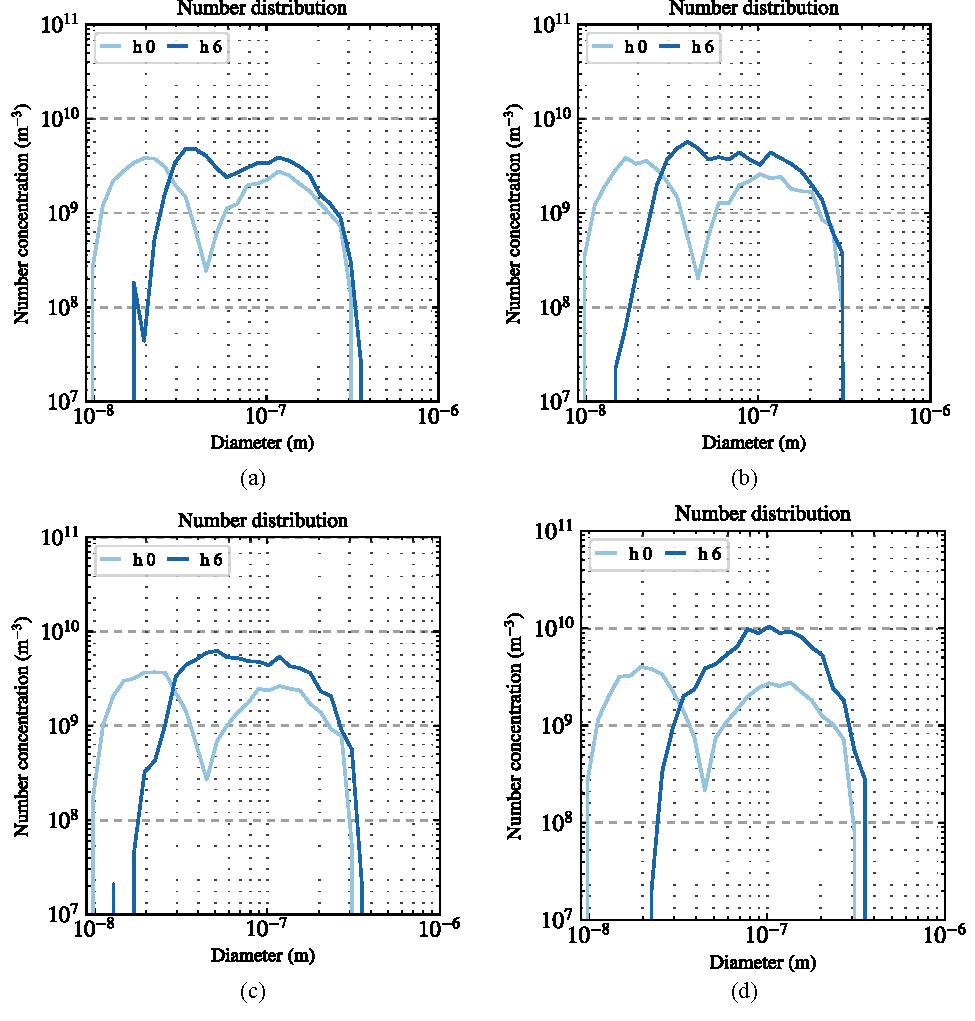
\includegraphics[width=\textwidth]{figures/chapter5/number-distribution-plots.pdf}
    \caption{}
    \label{fig:number-dists}
\end{figure}

\begin{figure}[t]
  \centering
    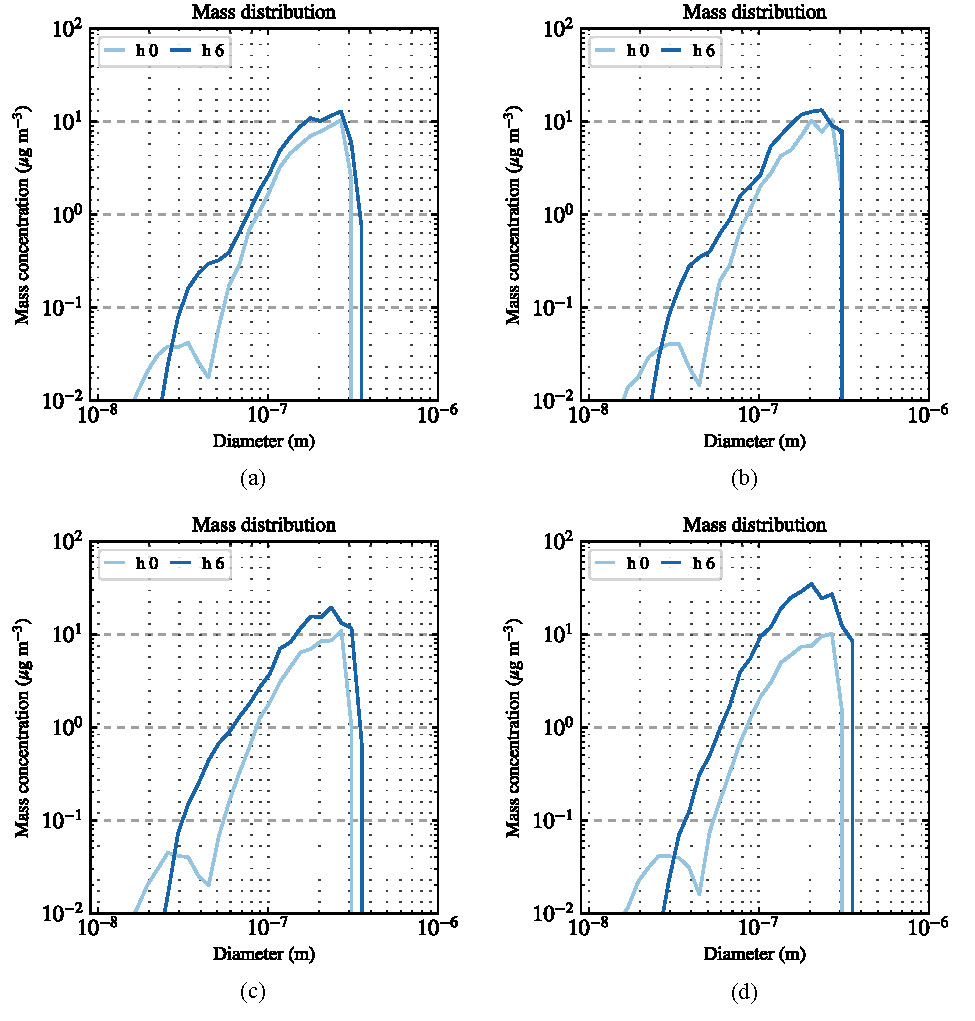
\includegraphics[width=\textwidth]{figures/chapter5/mass-distribution-plots.pdf}
    \caption{}
    \label{fig:mass-dists}
\end{figure}


\subsection{aerosol composition}

\begin{itemize}
\item Time-height plots for sulfate, nitrate, ammonium
\item \% mass fraction vs particle diameter plots
\item kappa distributions (either here or in the ccn subsection?)
\end{itemize}

\subsection{aerosol mixing state}

\begin{itemize}
\item Vertical profile of average particle $\chi$, $D_{\alpha}$, $D_{\gamma}$
\item Vertical profile of ccn $\chi$, $D_{\alpha}$, $D_{\gamma}$
\end{itemize}

\subsection{ccn}

\begin{itemize}
\item Vertical profile of ccn conc at each supersaturation level
\item Vertical profile of ccn $\chi$, $D_{\alpha}$, $D_{\gamma}$
\item time height plots of ccn \% error
\item (potentially) some sort of box plot ccn error thing similar to what I showed at IAMA?
\end{itemize}

\subsection{Runs without ammonia}

\begin{itemize}
\item Vertical profile of SNA
\item Vertical profile of ccn conc at each supersaturation level
\end{itemize}

\newpage
\begin{figure}[h]
  \centering
    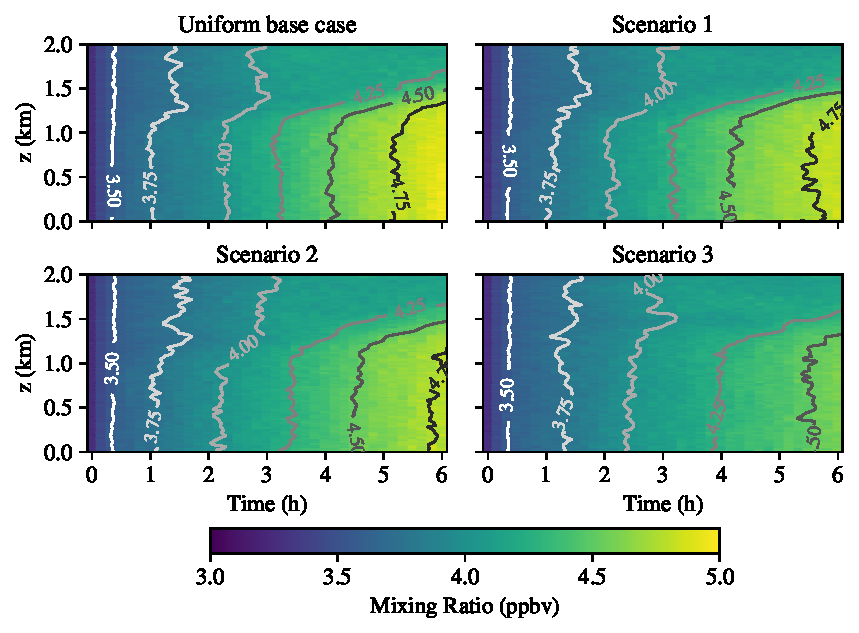
\includegraphics[width=\textwidth]{figures/chapter5/height-time-pmc_SO4-four-scenarios.pdf}
    \caption{Sulfate}
    \label{fig:ht-so4}
\end{figure}

\newpage
\begin{figure}[h]
  \centering
    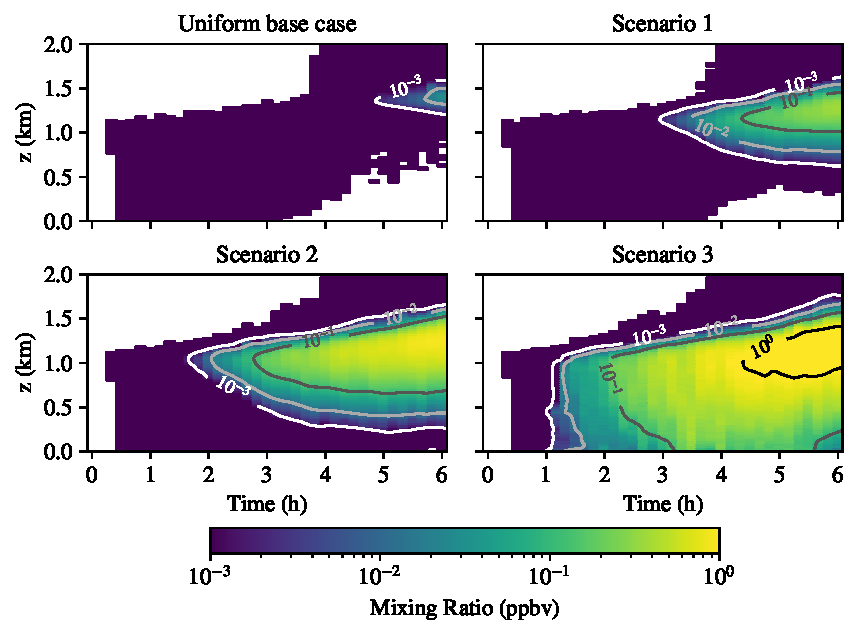
\includegraphics[width=\textwidth]{figures/chapter5/height-time-pmc_NO3-four-scenarios.pdf}
    \caption{Nitrate}
    \label{fig:ht-no3}
\end{figure}

\newpage
\begin{figure}[h]
  \centering
    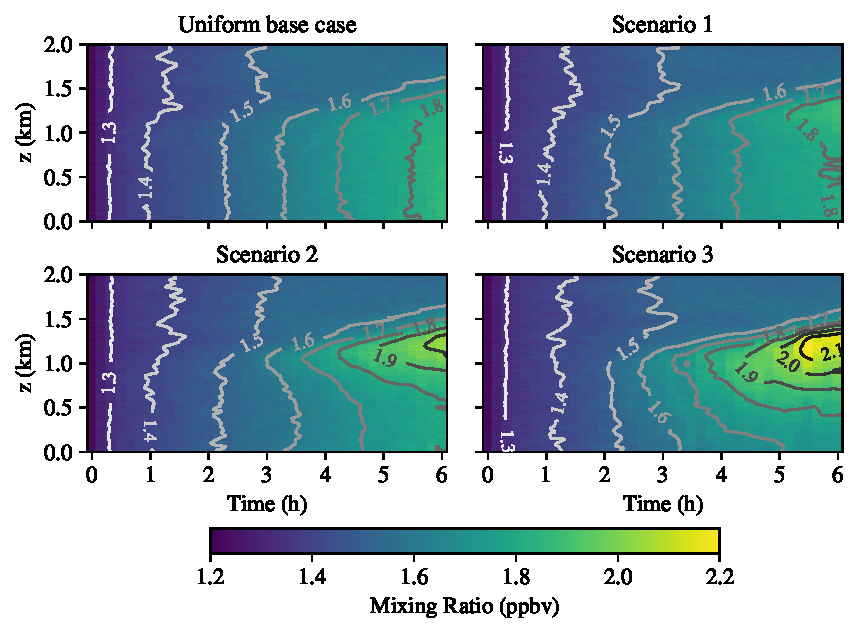
\includegraphics[width=\textwidth]{figures/chapter5/height-time-pmc_NH4-four-scenarios.pdf}
    \caption{Ammonium}
    \label{fig:ht-nh4}
\end{figure}


\newpage
\begin{figure}[h]
  \centering
    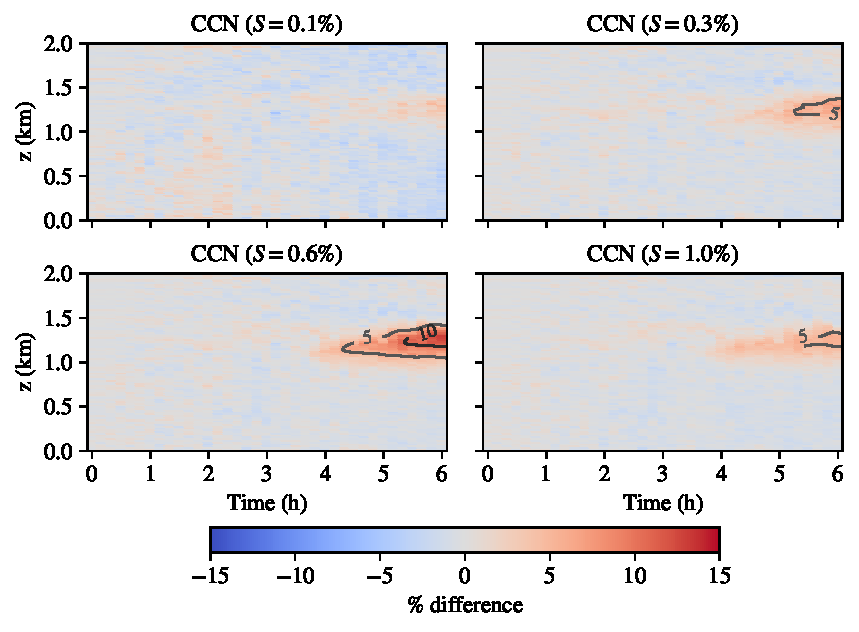
\includegraphics[width=\textwidth]{figures/chapter5/height-time-ccn-pdiff-fx1fy0.pdf}
    \caption{Scenario 1}
    \label{fig:ht-ccn-pdiff-s1}
\end{figure}

\newpage
\begin{figure}[h]
  \centering
    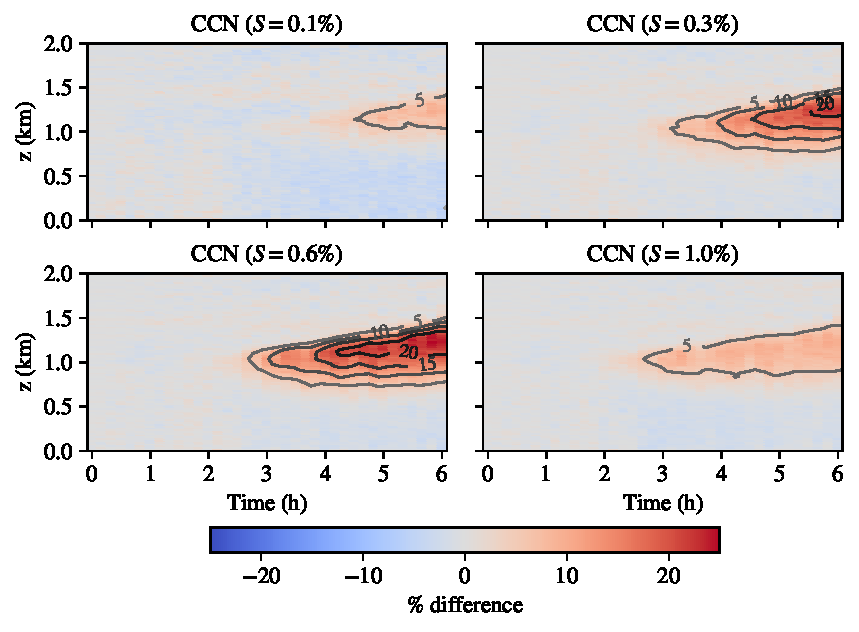
\includegraphics[width=\textwidth]{figures/chapter5/height-time-ccn-pdiff-road-10x.pdf}
    \caption{Scenario 2}
    \label{fig:ht-ccn-pdiff-s2}
\end{figure}

\newpage
\begin{figure}[h]
  \centering
    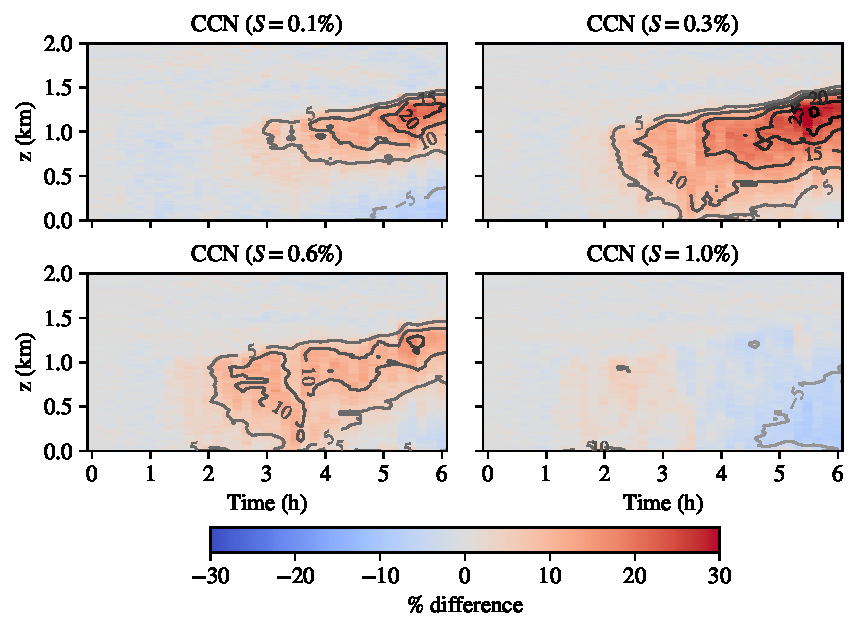
\includegraphics[width=\textwidth]{figures/chapter5/height-time-ccn-pdiff-point-source-1x1.pdf}
    \caption{Scenario 3}
    \label{fig:ht-ccn-pdiff-s3}
\end{figure}

